\documentclass{article}
\usepackage{amsmath}
\usepackage{amssymb}
\usepackage{amsthm}
\usepackage{graphicx}
\usepackage{listings}
\usepackage{xcolor}
\usepackage{float}

% Define listing style for code presentation
\definecolor{codegreen}{rgb}{0,0.6,0}
\definecolor{codegray}{rgb}{0.5,0.5,0.5}
\definecolor{codepurple}{rgb}{0.58,0,0.82}
\definecolor{backcolour}{rgb}{0.95,0.95,0.92}

\lstdefinestyle{mystyle}{
    backgroundcolor=\color{backcolour},
    commentstyle=\color{codegreen},
    keywordstyle=\color{magenta},
    numberstyle=\tiny\color{codegray},
    stringstyle=\color{codepurple},
    basicstyle=\ttfamily\footnotesize,
    breakatwhitespace=false,
    breaklines=true,
    captionpos=b,
    keepspaces=true,
    numbers=left,
    numbersep=5pt,
    showspaces=false,
    showstringspaces=false,
    showtabs=false,
    tabsize=2
}

\lstset{style=mystyle}

\title{Rapport du mini-projet capteur-actionneur avec STM32}
\author{AVRIL Théo, LERISSEL Elouen}
\date{\today}

\begin{document}
\maketitle
\tableofcontents

\section{Introduction}
\subsection{Contexte}
Dans le cadre de notre formation, nous avons développé un système embarqué utilisant un microcontrôleur STM32F411RE et une RaspberryPi 3b+.

\subsection{Objectif}
L'objectif principal était de développer un système fonctionne incluant une STM32 et une RaspberryPi.
Le système est capable de :
\begin{itemize}
    \item Retourner la distance mesurée par le capteur ultrasonique HC-SR04 sur une interface de commande sur la Raspberry Pi.
    \item Controler le servomoteur connecté sur la STM32 depuis une interface de commande sur la Raspberry Pi.
    \item De controler en automatique les deux servomoteurs en fonction de la distance mesurée par le capteur ultrasonique au travers d'un calcul réalisé sur la RaspberryPi.
\end{itemize}

Pour cela, la STM32 doit être configurée pour :
\begin{itemize}
    \item Mesurer une distance avec le capteur HC-SR04 toutes les 250 ms
    \item Communiquer les informations de distance via la liaison série toutes les 250 ms
    \item Recevoir une consigne de position pour le servomoteur via la liaison série et l'appliquer au servomoteur
\end{itemize}

Et la Raspberry Pi doit être configurée pour :
\begin{itemize}
    \item Recevoir la distance mesurée par la STM32 via la liaison série
    \item Envoyer une consigne de position pour le servomoteur à la STM32 via la liaison série
    \item Calculer la position de son servomoteur en fonction de la distance mesurée par le capteur ultrasonique
    \item Envoyer la position calculée au servomoteur de la STM32 via la liaison série
\end{itemize}



\section{Brochage des différents éléments}

\subsection{Capteur ultrasonique HC-SR04}
\begin{itemize}
    \item \textbf{VCC} : Alimentation 5V
    \item \textbf{GND} : Masse
    \item \textbf{TRIG} : Pin PB7 (TIM4\_CH2) - Signal de déclenchement
    \item \textbf{ECHO} : Pin connecté au GPIO en mode interruption externe (EXTI)
\end{itemize}

\subsection{Servomoteur}
\begin{itemize}
    \item \textbf{VCC} : Alimentation 5V
    \item \textbf{GND} : Masse
    \item \textbf{SIGNAL} : Pin PB5 (TIM3\_CH2) - Signal PWM
\end{itemize}

\subsection{LEDs de signalisation}
\begin{itemize}
    \item \textbf{LED bleue} : Indique le mode 1 (servo contrôlé par distance)
    \item \textbf{LED verte} : Indique le mode 2 (servo contrôlé par liaison série)
\end{itemize}

\subsection{Communication série UART}
\begin{itemize}
    \item \textbf{USART2\_TX} : Pin PA2 - Transmission de données
    \item \textbf{USART2\_RX} : Pin PA3 - Réception de données
\end{itemize}


\section{Configuration des périphériques internes}

\subsection{Timer et génération PWM}

\subsubsection{Timer pour la mesure de distance (TIM4)}
Nous avons configuré le TIM4 pour générer la pulsation de 10 µs nécessaire au déclenchement du capteur HC-SR04 toutes les 250 ms. Comme détaillé dans notre calcul initial:

\begin{lstlisting}[caption={Configuration du TIM4}, label={lst:tim4config}]
htim4.Instance = TIM4;
htim4.Init.Prescaler = 319;
htim4.Init.CounterMode = TIM_COUNTERMODE_UP;
htim4.Init.Period = 65535;
htim4.Init.ClockDivision = TIM_CLOCKDIVISION_DIV1;
htim4.Init.AutoReloadPreload = TIM_AUTORELOAD_PRELOAD_DISABLE;
\end{lstlisting}

Un signal PWM avec un rapport cyclique très court (10µs) est généré sur le canal 2 pour déclencher le capteur ultrasonique.

\subsubsection{Timer pour le servomoteur (TIM3)}
Le TIM3 est configuré pour générer un signal PWM adapté au contrôle du servomoteur:

\begin{lstlisting}[caption={Configuration du TIM3}, label={lst:tim3config}]
htim3.Instance = TIM3;
htim3.Init.Prescaler = 28;
htim3.Init.CounterMode = TIM_COUNTERMODE_UP;
htim3.Init.Period = 59999;
htim3.Init.ClockDivision = TIM_CLOCKDIVISION_DIV1;
htim3.Init.AutoReloadPreload = TIM_AUTORELOAD_PRELOAD_DISABLE;
\end{lstlisting}

Cette configuration génère un signal PWM avec une période de 20 ms (50 Hz), ce qui est la fréquence standard pour contrôler les servomoteurs.

\subsection{Configuration des interruptions EXTI}
Pour mesurer précisément le temps de vol des ondes ultrasoniques, nous avons utilisé les interruptions externes (EXTI) pour détecter les fronts montants et descendants du signal ECHO retourné par le capteur HC-SR04.

\begin{lstlisting}[caption={Callback d'interruption EXTI}, label={lst:exticallback}]
void gpio_trigger_Callback() {
    static uint32_t start_time = 0;
    // Lecture de l'etat du pin
    int8_t echo = HAL_GPIO_ReadPin(SonicSensor_Echo_GPIO_Port, SonicSensor_Echo_Pin);
    if (echo){
        // Enregistrement du temps de debut
        start_time = HAL_GetTick();
    } else {
        // Calcul de la duree
        uint32_t duration = HAL_GetTick() - start_time;
        // Calcul de la distance en cm
        distance = (duration * 340)/100/2;
    }
}
\end{lstlisting}

\subsection{Configuration UART}
La communication série est configurée pour permettre l'envoi de la distance mesurée et la réception des commandes de changement de mode ou de position du servomoteur.

\begin{lstlisting}[caption={Initialisation UART}, label={lst:uartinit}]
MX_USART2_UART_Init();
HAL_UART_Transmit(&huart2, (uint8_t *)"Hello World\r\n", 13, HAL_MAX_DELAY);
\end{lstlisting}



\section{Modules développés}

\begin{figure}[H]
    \centering
    \includegraphics[width=12cm]{diagram/class_diagram.png}
    \caption{Diagramme de classe du projet \newline \textit{N'include que les module développé par nos soins}}
    \label{fig:class_diagram}
\end{figure}

\subsection{Module capteur ultrasonique (ULTRA\_SONIC)}
Ce module implémente un pattern Singleton pour gérer le capteur HC-SR04. Il offre les fonctionnalités suivantes:

\begin{lstlisting}[caption={Module capteur ultrasonique}, label={lst:ultrasonicmodule}]
void ULTRA_SONIC_Init(void)
{
    // Initialisation du capteur ultrasonique
    HAL_TIM_PWM_Start(&htim4, TIM_CHANNEL_2);
    GPIO_RegisterGPIO_EXTICallback(gpio_trigger_Callback, SonicSensor_Echo_Pin);
}

float ULTRA_SONIC_GetDistance(void)
{
    return distance; 
}

void ULTRA_SONIC_test(void){
    float distance = ULTRA_SONIC_GetDistance();
    char buffer[50];
    int len = snprintf(buffer, sizeof(buffer), "Distance: %f \r\n", distance);
    HAL_UART_Transmit(&huart2, (uint8_t *)buffer, len, HAL_MAX_DELAY);
    HAL_Delay(1000);
}
\end{lstlisting}

Le principe de fonctionnement est le suivant:
\begin{enumerate}
    \item Envoi d'une impulsion de 10 µs sur le pin TRIG
    \item Attente du signal ECHO et mesure de sa durée via interruption
    \item Calcul de la distance selon la formule: $distance = \frac{duree \times vitesse\_son}{2}$
\end{enumerate}

\subsection{Module servomoteur (SERVO)}
Ce module implémente également un pattern Singleton pour gérer le servomoteur:

\begin{lstlisting}[caption={Module servomoteur}, label={lst:servomodule}]
#define MIN_DUTY 2000
#define MAX_DUTY 4000

void SERVO_Init(void)
{
    // Initialisation du servomoteur
    HAL_TIM_PWM_Start(&htim3, TIM_CHANNEL_2);
    __HAL_TIM_SetCompare(&htim3, TIM_CHANNEL_2, MIN_DUTY);
}

void SERVO_set_servo_percentage(uint8_t percentage)
{
    // Configuration du rapport cyclique selon le pourcentage
    uint32_t duty_cycle = MIN_DUTY + (MAX_DUTY - MIN_DUTY) * percentage / 100;
    __HAL_TIM_SetCompare(&htim3, TIM_CHANNEL_2, duty_cycle);
}
\end{lstlisting}

Le servomoteur est contrôlé par un signal PWM dont la largeur d'impulsion détermine la position angulaire:
\begin{itemize}
    \item MIN\_DUTY (2000) correspond à la position 0°
    \item MAX\_DUTY (4000) correspond à la position 180°
\end{itemize}

\subsection{Module LED (LEDS)}
Un module simple pour gérer les LEDs d'indication de mode:

\begin{lstlisting}[caption={Interface du module LED}, label={lst:ledmodule}]
void LEDS_Init(void);
void LEDS_SetMode(uint8_t mode);
\end{lstlisting}

\subsection{Module communication série}
Le module de communication série permet d'envoyer la distance mesurée et de recevoir les commandes:

\begin{lstlisting}[caption={Exemple de communication série}, label={lst:serialcomm}]
// Envoi de la distance
float distance = ULTRA_SONIC_GetDistance();
char buffer[50];
int len = snprintf(buffer, sizeof(buffer), "Distance: %f \r\n", distance);
HAL_UART_Transmit(&huart2, (uint8_t *)buffer, len, HAL_MAX_DELAY);
\end{lstlisting}

\subsection{Module bouton poussoir (BUTTON)}
Le module de gestion du bouton poussoir permet de changer le mode de fonctionnement du système. Il utilise une interruption externe pour détecter les pressions sur le bouton:

Le module BUTTON gère un bouton poussoir de manière autonome en utilisant une interruption externe. Il se base sur deux variables globales principales : une variable indiquant si le bouton a été pressé et une autre mémorisant le dernier instant d’activation, ce qui est crucial pour le contrôle du rebond.

\begin{enumerate}
    \item Gestion du rebond
    \begin{itemize}
        \item Lorsqu'une pression sur le bouton est détectée, une interruption est générée.
        \item La fonction de rappel vérifie si l'intervalle écoulé depuis le dernier appui dépasse un seuil (200 ms).
        \item Si le délai n'est pas respecté, l'appui est ignoré pour éviter les faux signaux.
    \end{itemize}
    \item Mise à jour de l’état et communication
    \begin{itemize}
        \item En cas d’appui valide, la fonction de rappel met à jour la variable d’état (passant à 1).
        \item Elle enregistre l’instant courant via un appel système (par exemple, HAL\_GetTick()).
        \item Un message est envoyé via l’interface UART pour notifier le reste du système de l’événement.
    \end{itemize}
    \item Initialisation et configuration
    \begin{itemize}
        \item Avant d’être opérationnel, le module doit être initialisé.
        \item Une fonction dédiée configure le bouton pour qu’il génère une interruption à chaque pression.
        \item Elle associe le pin correspondant au bouton à la fonction de rappel, garantissant ainsi que l’appui sur le bouton déclenche automatiquement la gestion d’événement.
    \end{itemize}
    \item Lecture et réinitialisation de l’état
    \begin{itemize}
        \item Une fonction de lecture permet à d'autres parties du programme de vérifier si le bouton a été pressé.
        \item Une fois l’événement traité, une fonction de réinitialisation remet la variable d’état à zéro pour préparer la détection de futures pressions.
    \end{itemize}
\end{enumerate}


\subsection{Schémas d'explication}

\subsubsection{Diagramme temporel du capteur HC-SR04}

\begin{figure}[H]
    \centering
    \begin{minipage}{0.45\textwidth}
        \centering
        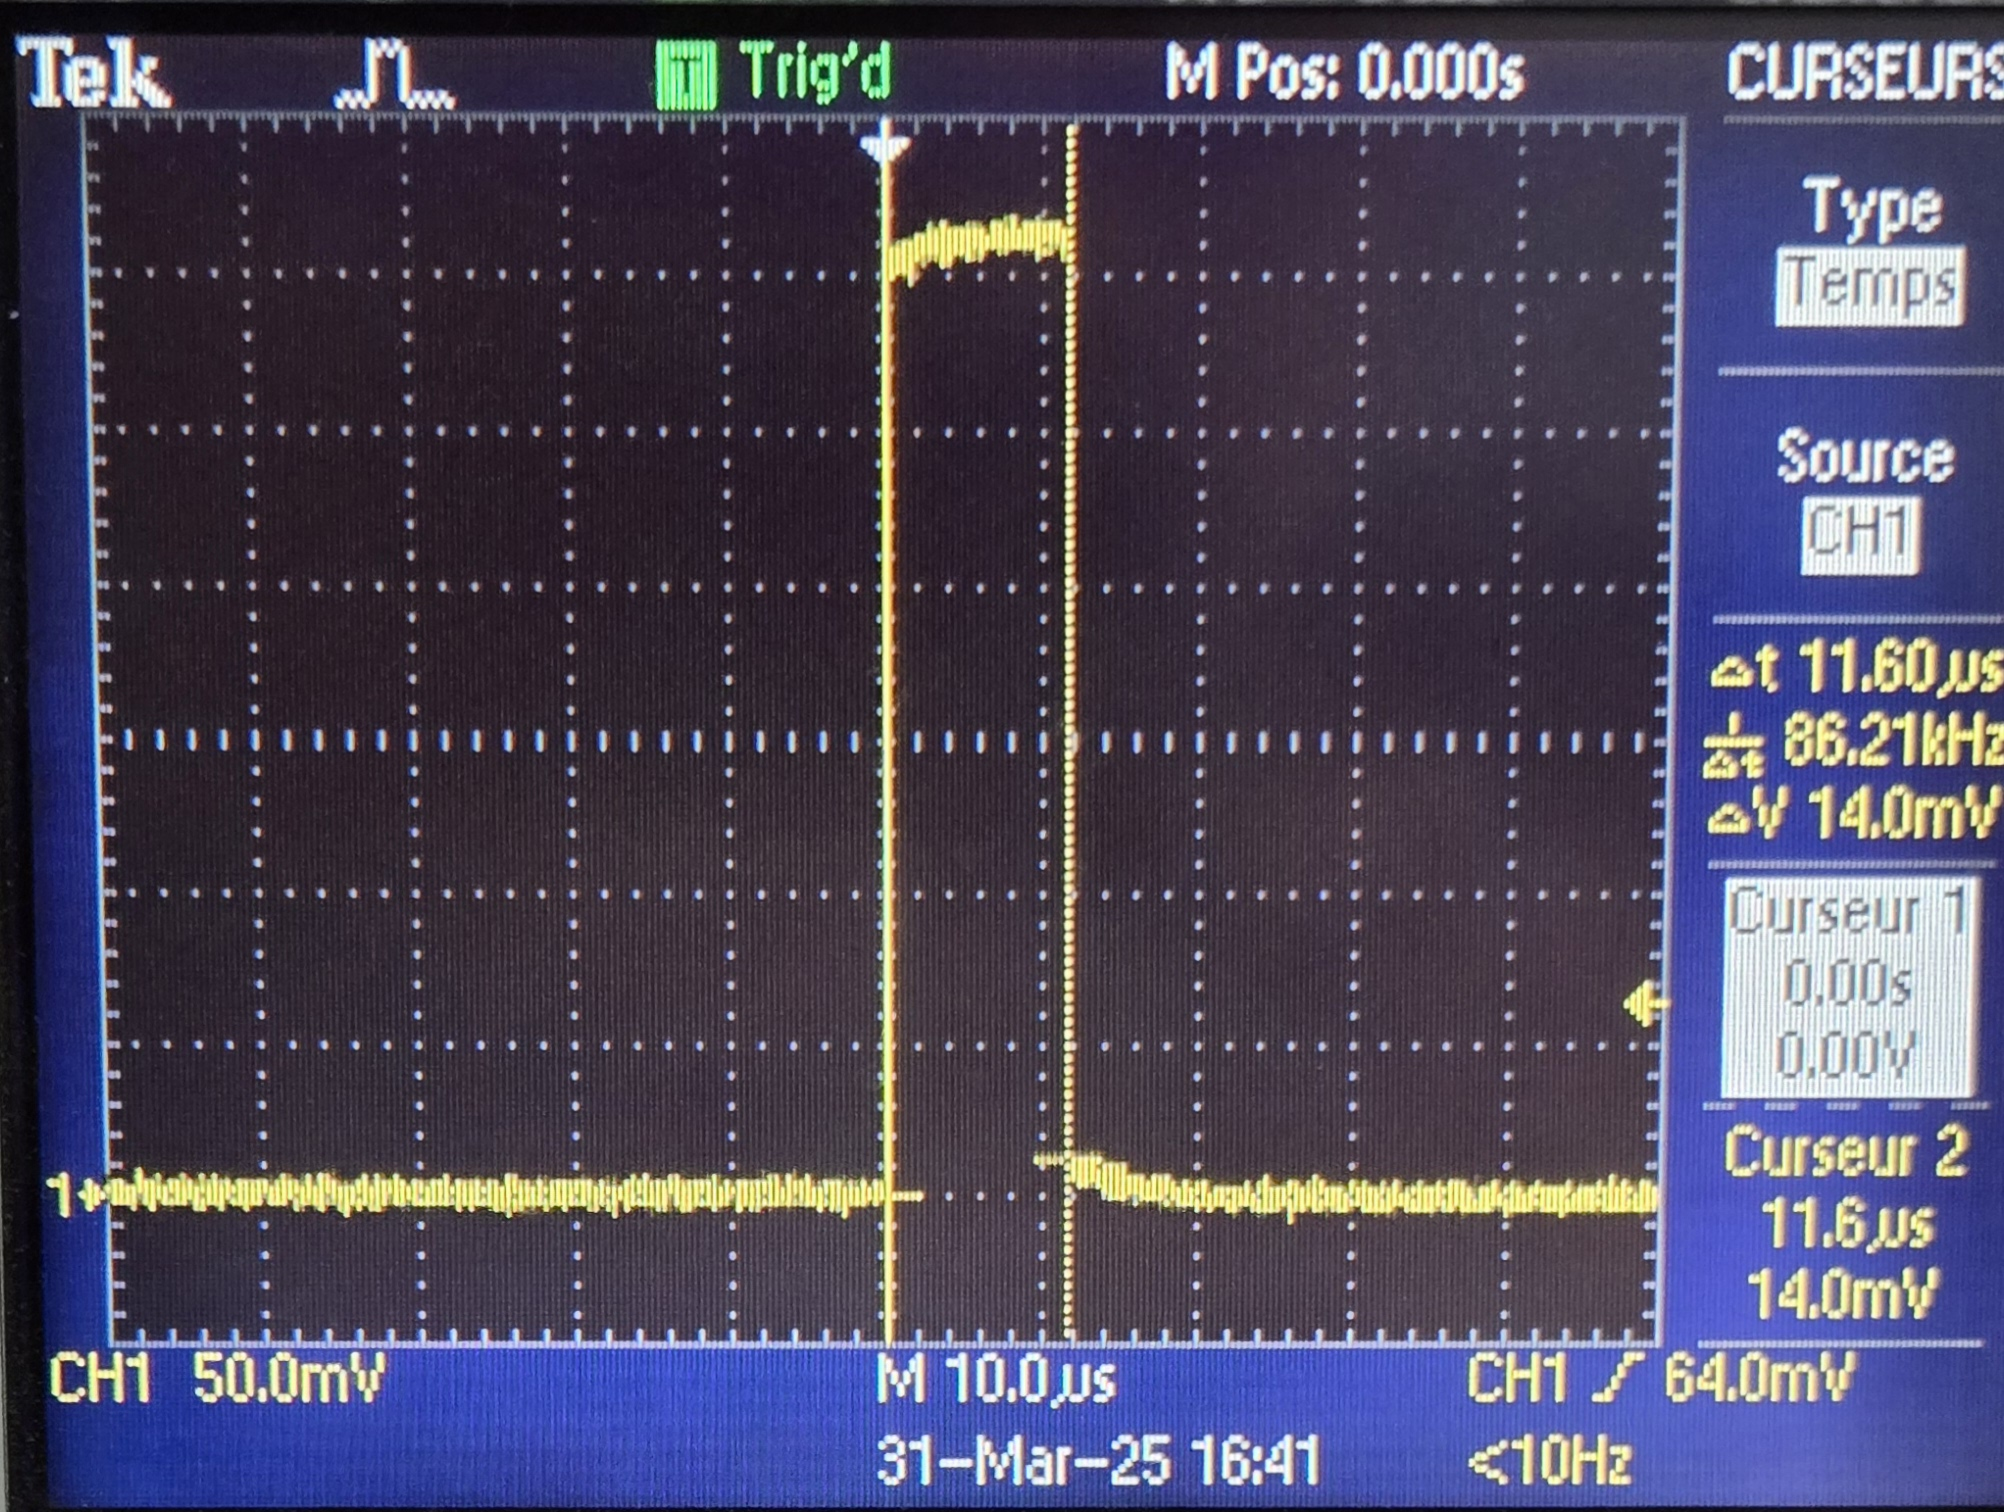
\includegraphics[width=\textwidth]{img/input_sr-04.jpg}
        \caption{Signal d'entrée du capteur HC-SR04 (TRIG)}
        \label{fig:input_sr-04}
    \end{minipage}
    \hfill
    \begin{minipage}{0.45\textwidth}
        \centering
        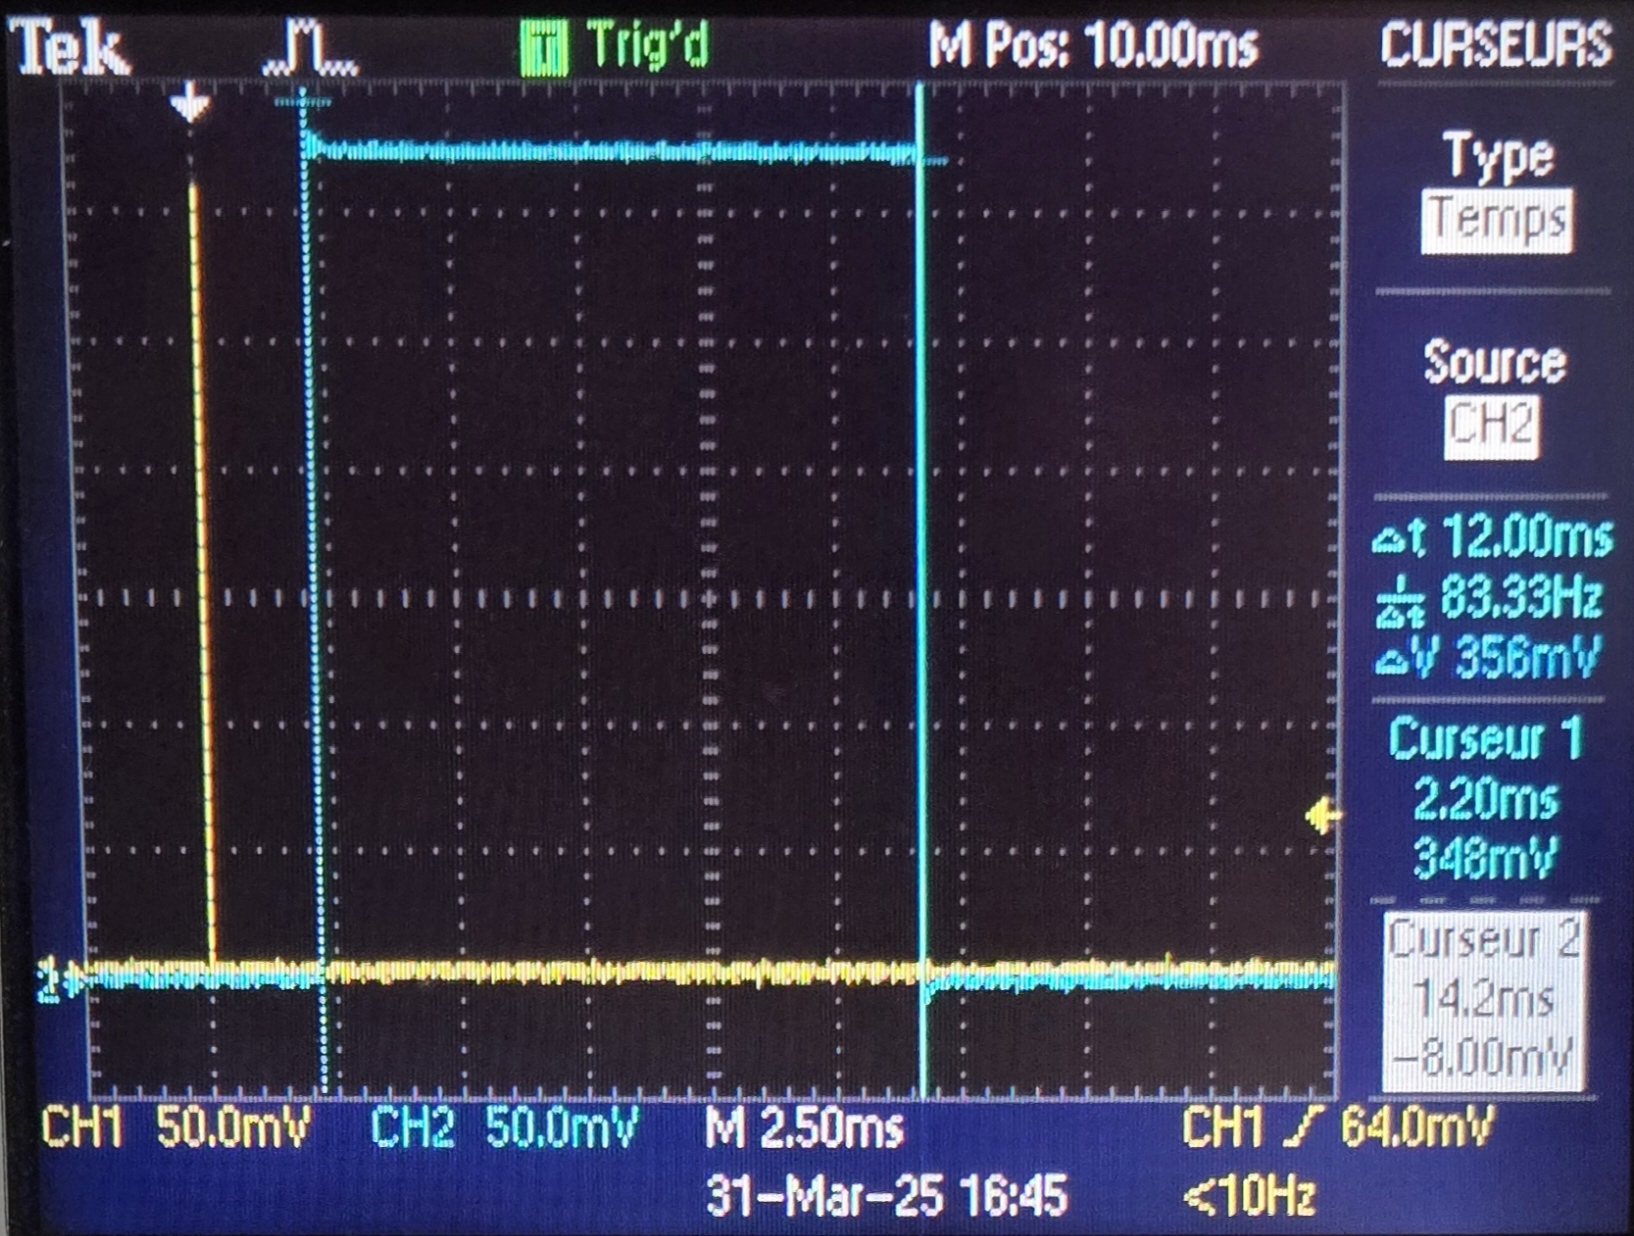
\includegraphics[width=\textwidth]{img/output_sr-04.jpg}
        \caption{Signal de sortie du capteur HC-SR04 (ECHO)}
        \label{fig:output_sr-04}
    \end{minipage}
\end{figure}

\subsubsection{Signal PWM du servomoteur}
\begin{figure}
    \centering
    \begin{minipage}
        {0.8\textwidth}
        \centering
        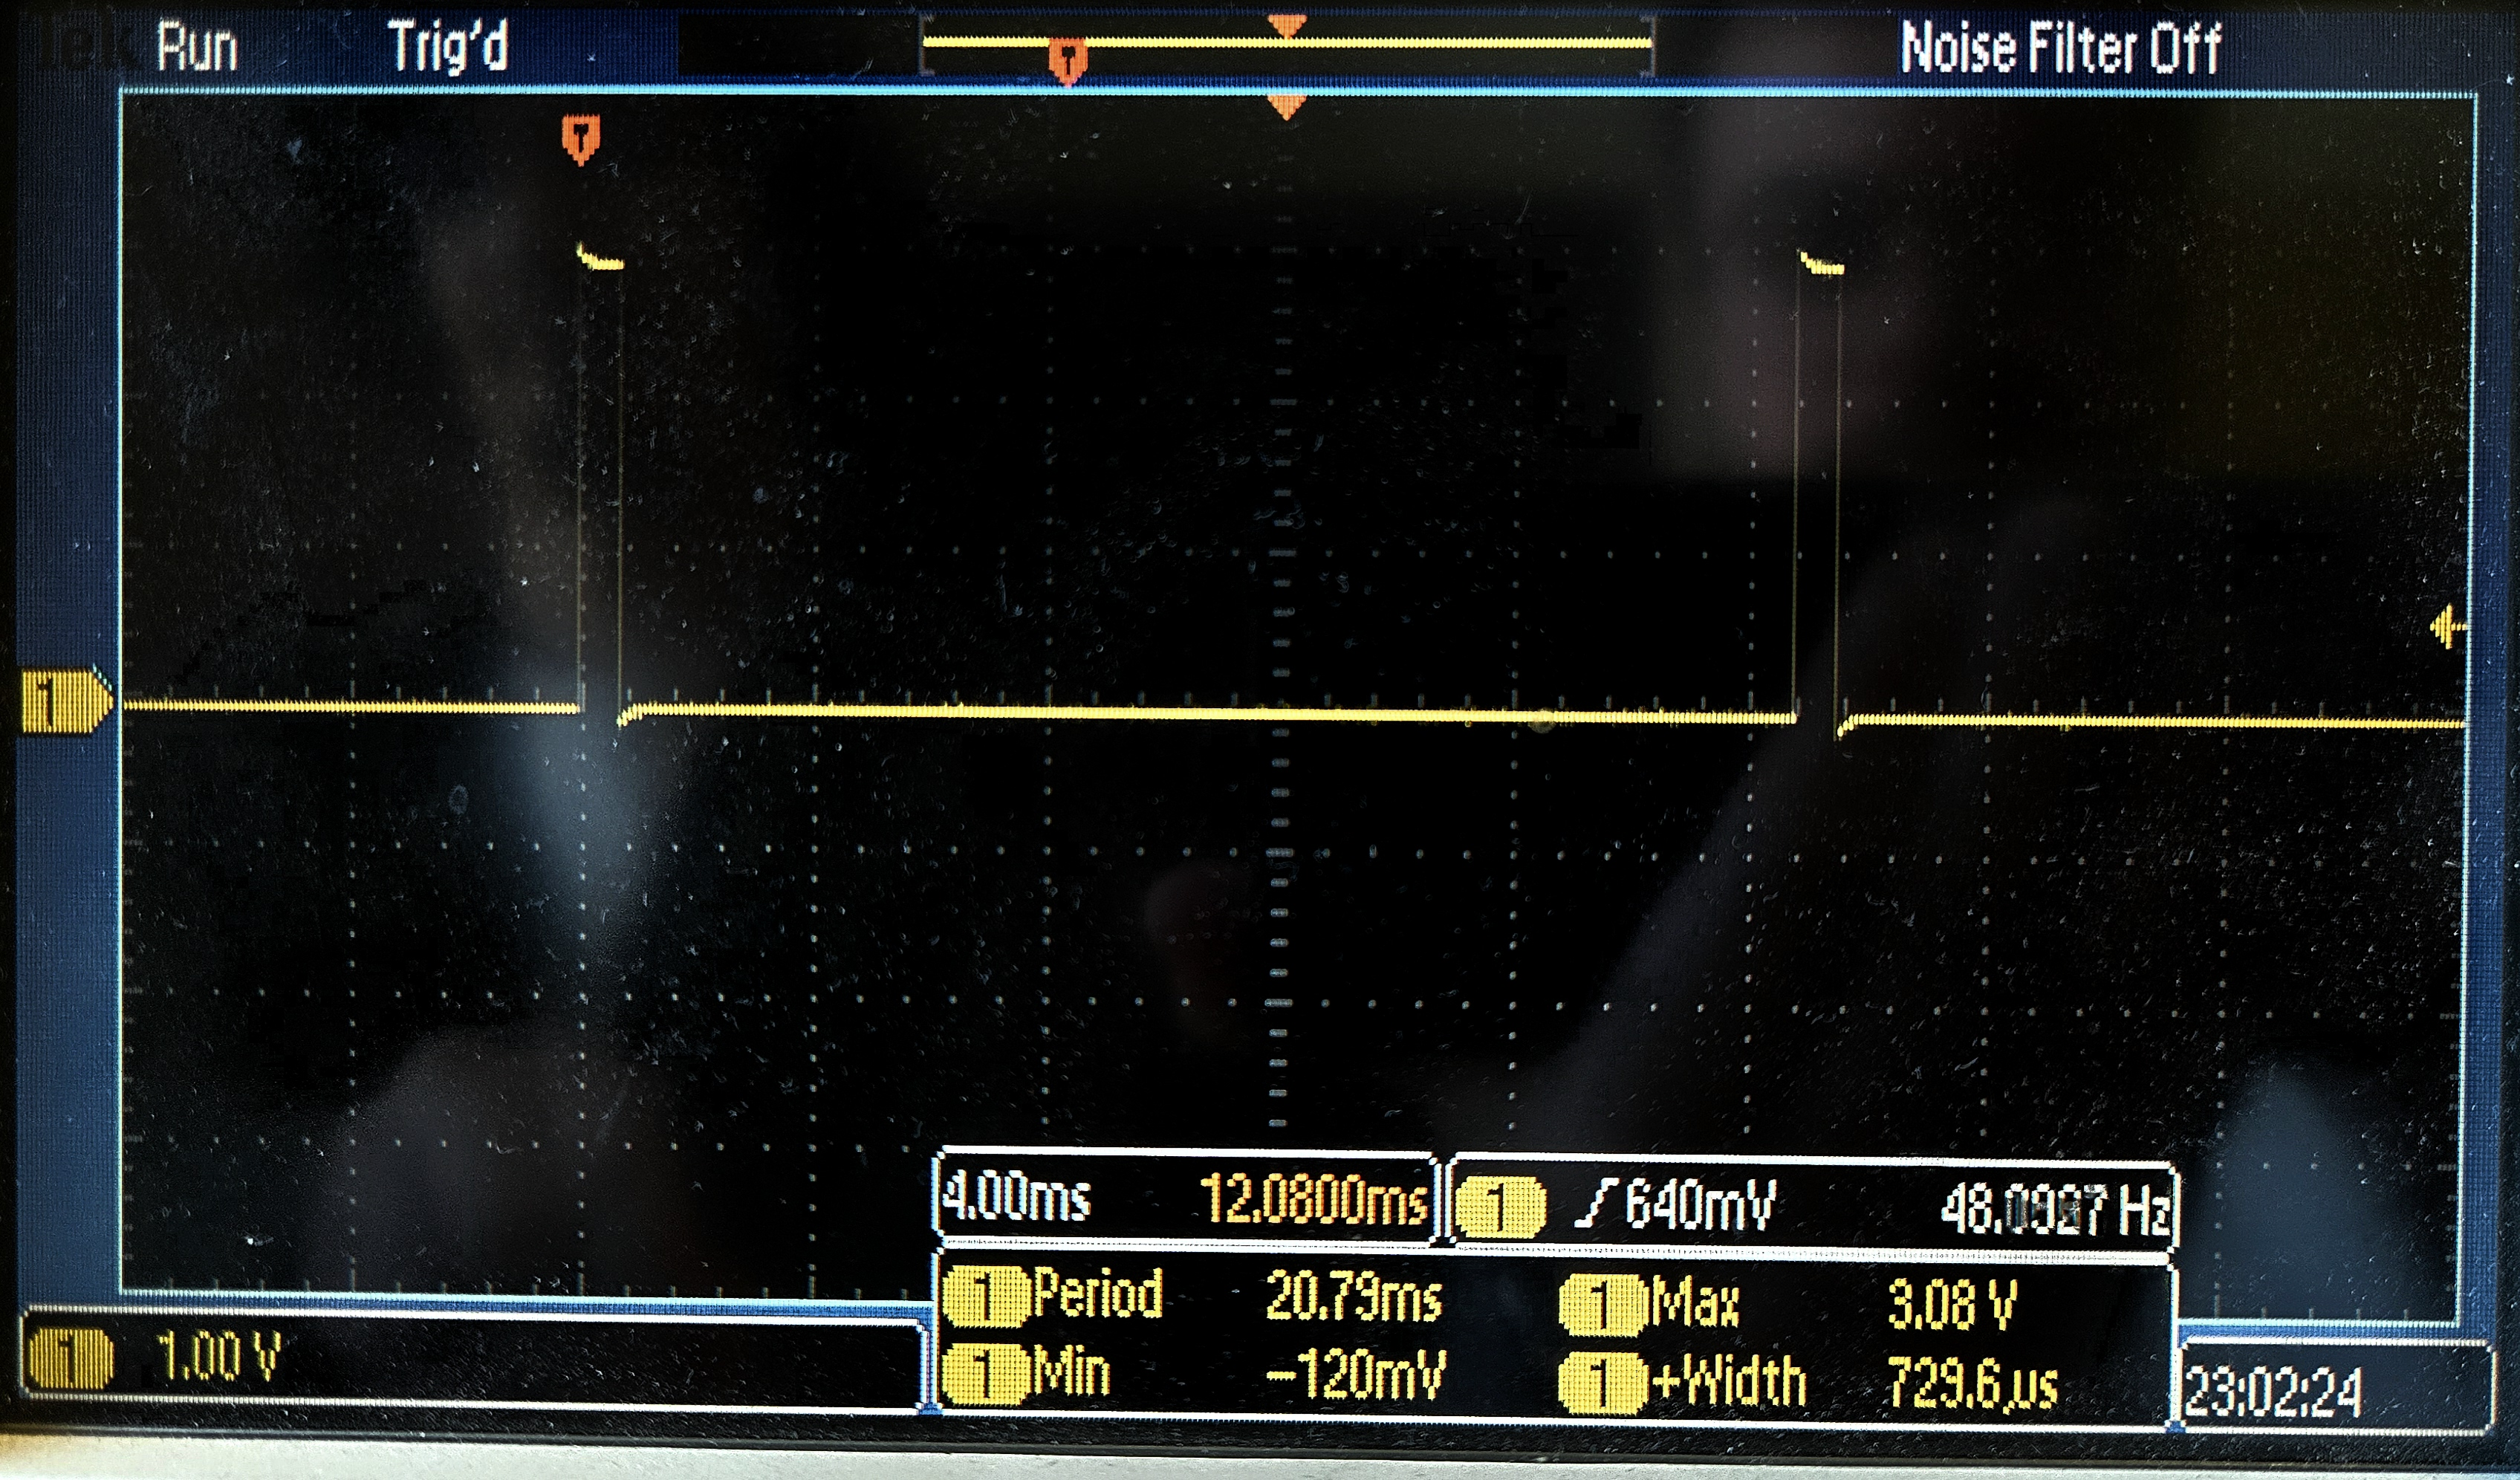
\includegraphics[width=\textwidth]{img/servo.jpg}
        \caption{Signal PWM du servomoteur}
        \label{fig:pwm_signal}
    \end{minipage}
\end{figure}


\section{Étapes de conception et validations associées}

\subsection{Mise en place du timer pour la mesure périodique}
Première étape: configurer un timer pour déclencher des mesures toutes les 250 ms.

\subsubsection{Calcul de la configuration}
Comme détaillé précédemment, pour obtenir une période de 250 ms avec une fréquence d'horloge de 84 MHz:
\begin{align*}
P &= \frac{(1 + \text{counter\_period}) \times (1 + \text{prescaler})}{F} \\
0,25 &= \frac{(1 + \text{counter\_period}) \times (1 + \text{prescaler})}{84 \times 10^6} \\
(1 + \text{counter\_period}) \times (1 + \text{prescaler}) &= 21~000~000
\end{align*}

Nous avons choisi:
\begin{itemize}
    \item counter\_period = 65535
    \item prescaler = 319
\end{itemize}

\subsubsection{Validation}
La validation a été effectuée en vérifiant la fréquence de déclenchement des mesures avec l'oscilloscope, confirmant une période de 249,66 ms, très proche des 250 ms visés.

\subsection{Développement du module HC-SR04}
\subsubsection{Principe de fonctionnement}
Le principe du capteur HC-SR04:
\begin{enumerate}
    \item Envoi d'une impulsion de 10 µs sur TRIG
    \item Le capteur émet 8 impulsions ultrasoniques à 40 kHz
    \item Le capteur place ECHO à l'état haut jusqu'au retour de l'onde réfléchie
    \item La durée de l'impulsion ECHO est proportionnelle à la distance
\end{enumerate}

\subsubsection{Mise en œuvre et validation}
\begin{itemize}
    \item Configuration d'un signal PWM très court (Pulse = 3) pour le déclenchement
    \item Utilisation des interruptions externes pour mesurer la durée du signal ECHO
    \item Calcul de la distance: $\text{distance} = \frac{\text{durée} \times 340 \text{ m/s}}{2}$
    \item Validation par comparaison avec une mesure de référence
\end{itemize}

\subsection{Développement du module servomoteur}
\subsubsection{Principe de fonctionnement}
Le servomoteur est contrôlé par un signal PWM de période 20 ms (50 Hz):
\begin{itemize}
    \item Largeur d'impulsion de 1 ms: position 0°
    \item Largeur d'impulsion de 2 ms: position 180°
\end{itemize}

\subsubsection{Mise en œuvre et validation}
\begin{itemize}
    \item Configuration du TIM3 pour générer un signal PWM à 50 Hz
    \item Implémentation d'une fonction pour convertir un pourcentage (0-100\%) en largeur d'impulsion
    \item Validation par observation du mouvement du servomoteur
\end{itemize}

\subsection{Implémentation des modes de fonctionnement}
\subsubsection{Mode 1: Contrôle par distance}
Dans ce mode, la position du servomoteur est proportionnelle à la distance mesurée:
\begin{lstlisting}[caption={Contrôle par distance}, label={lst:mode1}]
float distance = ULTRA_SONIC_GetDistance();
uint8_t percentage = (uint8_t)(distance / 21 * 100);
SERVO_set_servo_percentage(percentage);
\end{lstlisting}

\subsubsection{Mode 2: Contrôle par commande série}
Dans ce mode, la position du servomoteur est définie par une commande reçue via la liaison série.

\subsection{Intégration du système complet}
L'intégration finale a consisté à:
\begin{itemize}
    \item Combiner tous les modules développés
    \item Implémenter la machine à états pour gérer les deux modes
    \item Gérer le changement de mode par bouton-poussoir ou commande série
    \item Transmettre périodiquement la distance mesurée
\end{itemize}


\section{Informations complémentaires}

\subsection{Tableau complet des connexions}
\begin{table}[H]
\centering
\begin{tabular}{|l|l|l|l|}
\hline
\textbf{Composant} & \textbf{Pin} & \textbf{Fonction} & \textbf{Configuration} \\
\hline
HC-SR04 Trigger & PB7 & Output & TIM4\_CH2 (PWM) \\
\hline
HC-SR04 Echo & PB8 & Input & EXTI (Rising/Falling) \\
\hline
Servo & PB5 & Output & TIM3\_CH2 (PWM) \\
\hline
LED Bleue & PD15 & Output & GPIO Push-Pull \\
\hline
LED Verte & PD12 & Output & GPIO Push-Pull \\
\hline
UART TX & PA2 & Output & USART2\_TX \\
\hline
UART RX & PA3 & Input & USART2\_RX \\
\hline
Bouton-poussoir & PA0 & Input & EXTI (Falling) \\
\hline
\end{tabular}
\caption{Récapitulatif des connexions matérielles}
\label{tab:connections}
\end{table}

\subsection{Gestion des erreurs}
Le système intègre une gestion basique des erreurs:
\begin{itemize}
    \item Vérification des mesures de distance (filtrage des valeurs aberrantes)
    \item Détection des timeouts pour le capteur ultrasonique
    \item Validation des commandes reçues via la liaison série
\end{itemize}

\subsection{Améliorations possibles}
Plusieurs améliorations pourraient être apportées:
\begin{itemize}
    \item Implémentation d'un filtre pour stabiliser les mesures de distance
    \item Développement d'une interface utilisateur plus complète
    \item Ajout de fonctionnalités de diagnostic et de calibration
    \item Utilisation du DMA pour optimiser les transferts UART
\end{itemize}

\section{Conclusion}
Ce mini-projet nous a permis de mettre en pratique plusieurs concepts importants:
\begin{itemize}
    \item Configuration et utilisation des timers et du PWM
    \item Gestion des interruptions externes
    \item Développement de modules réutilisables (pattern Singleton)
    \item Communication série
    \item Interfaçage avec des composants externes (capteur et servomoteur)
\end{itemize}

Le système développé répond aux exigences initiales en permettant de mesurer des distances et de contrôler un servomoteur selon deux modes distincts. L'architecture modulaire adoptée facilite la maintenance et l'évolution future du projet.


\end{document}